% !TEX TS-program = pdflatex
% !TEX encoding = UTF-8
% !BIB program = biber

\documentclass[12pt,a4paper]{report}

% generira bookmarkove
\usepackage{bookmark}

% Podrška za hrvatski
\usepackage[croatian]{babel}
\usepackage{csquotes}

% Margine
\usepackage[left=3cm,top=2.5cm,right=2.5cm,bottom=3.5cm]{geometry}

% Simboli i naredbe za matematiku
\usepackage{amsmath, amsthm, amssymb}
\usepackage{mathtools}
\usepackage{subcaption} % side-by-side grafovi

%\usepackage{easyfig} % H fiksacija figura
\usepackage{pdflscape} % landscape stranice
\usepackage{spverbatim} % line break verbatim

% Podrška za slike
\usepackage{graphicx} % \includegraphics [k=v] interface

% Poveznice
\usepackage{hyperref}

% Blokovi s kodom
\usepackage{minted}
\ifx\write18\relax\else
\usemintedstyle{sas}
\fi

% Literatura
\usepackage[sorting=none,backend=biber,style=numeric]{biblatex}
\addbibresource{seminar.bib}

% Fonts:
\usepackage[T1]{fontenc} % Allows specifying fonts
\usepackage{helvet} % Helvetica; phv
\usepackage{palatino} % Palatino; ppl

\gdef \title{Wordel}
\gdef \class{Objektno Programiranje}
\gdef \author{Tin Švagelj}
\gdef \uniprogram{Preddimplski studij informatike}
\gdef \semguide{
    Doc. dr. sc. Miran Pobar\\
    Mag. inf. et educ. inf. Ivona Franković
}
\gdef \author{Tin Švagelj}
\gdef \date{\today}

% Custom commands and redefinitions
\newcommand{\UseFont}[1]{\fontfamily{#1}\selectfont}

\usepackage{titlesec}
\titleformat{\chapter}[hang]
{\normalfont\Large\bfseries}{\thechapter}{20pt}{\Large}

% \usepackage{fancyhdr}
% \pagestyle{fancy}
% \fancyhead{}
% \renewcommand\headrulewidth{0.1pt}
% \fancyhead[L]{\footnotesize \leftmark}
% \fancyhead[R]{\footnotesize \thepage}
% \renewcommand\headrulewidth{0pt}
% \fancyfoot[R]{\small Fakultet Informatike i\\Digitalnih Tehnologija}
% \renewcommand\footrulewidth{0.1pt}
% \fancyfoot[C]{2022 - 2023}
% \fancyfoot[L]{\small \title}

\begin{document}

\thispagestyle{empty}

\begin{titlepage}
	\begin{center}
        {
            \bf
            FAKULTET INFORMATIKE I\\
            DIGITALNIH TEHNOLOGIJA\\
            \vspace{2pt}\uniprogram
        }

		\vspace*{\stretch{0.5}}
        {\LARGE Projektna dokumentacija iz kolegija}\\
        \vspace{8pt}{\LARGE \class}\\
		\vspace{16pt}{\UseFont{phv} \Huge \bf \title}
        \vspace*{\stretch{0.5}}
	\end{center}

    {
        \renewcommand{\arraystretch}{1.5}
        \begin{tabular}{l l}
            {\bf Autor:} & {\bf \author} \\
            {Mentor/ica:} & \parbox[t]{\columnwidth}{\semguide} \\
        \end{tabular}
    }

    \vspace*{\stretch{0.25}}
	\begin{center}
		{U Rijeci, \today}
	\end{center}
\end{titlepage}


\pagenumbering{roman}

\tableofcontents
\newpage

\pagenumbering{arabic}
\setcounter{page}{1}

\chapter{Uvod}

\begin{figure}
\centering
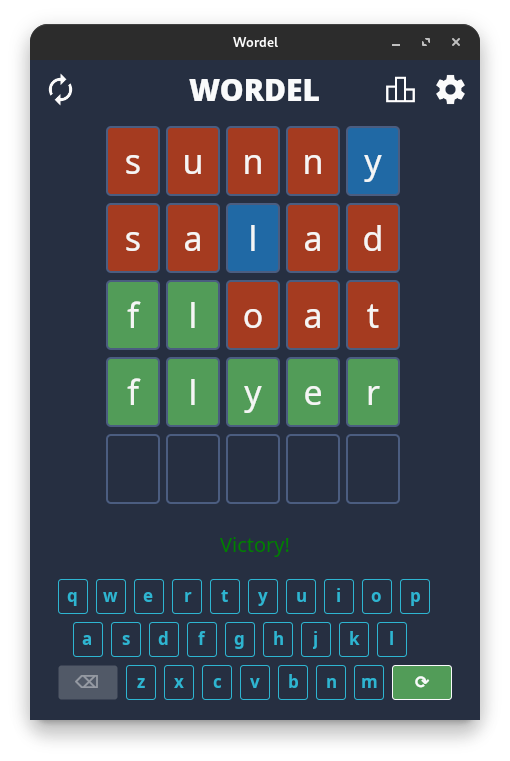
\includegraphics{../img/preview.png}
\caption{Prikaz aplikacije}
\end{figure}

{
    \raggedright

    GitHub:
    \href{https://github.com/Caellian/UNIRI_OP_project}{Caellian/UNIRI\_OP\_project}
    
    Dokumentacija:
    (\href{https://github.com/Caellian/UNIRI_OP_project/raw/main/tin_svagelj.pdf}{pdf}\textbar{}\href{https://github.com/Caellian/UNIRI_OP_project/raw/main/tin_svagelj.docx}{docx})    
}
\bigskip

\par
Cilj ovog rada je bio napraviti repliku web aplikacije
\href{https://www.nytimes.com/games/wordle/index.html}{Wordle} koju je
napravio \emph{The New York Times}.

\par
\href{https://dotnet.microsoft.com/en-us/apps/maui}{.NET Multi-platform
App UI} (nadalje MAUI) nije bio dobar odabir s obzirom da je za razvojno
okruženje bio korišten \emph{Linux} jer (trenutno) podržava samo MacOS i
Windows.

\par
Za izradbu su korišteni C\# programski jezik i
\href{https://avaloniaui.net/}{Avalonia UI} (nadalje AUI) platforma
(engl. framework) za razvoj korisničkog sučelja. Avalonia UI podržava
Windows, MacOS i Linux desktop operativne sustave, kao i iOS i Android,
te uz njih i WebAssembly (web preglednike). Površinom pokrivenosti
podržanih platformi je time sličnija \href{https://openjfx.io/}{JavaFX}
platformi koja je prethodno bila dio jezgrenog Java kompleta za razvoj
softvera (engl. Java SDK), dok ju Oracle nije odlučio ukloniti kako bi
smanjili veličinu JDKa povodom uvođenja modula.

\par
\hypertarget{ucitavanje-resursa-ukljucenih-u-projekt}{%
\chapter{Učitavanje resursa uključenih u
projekt}\label{ucitavanje-resursa-ukljucenih-u-projekt}}

\par
Dok se za rad s datotekama izmjenjivog sadržaja može koristiti
\verb|System.IO.File|, u kontekstu razvoja softvera često želimo
uključiti datoteke za koje ne očekujemo izmjene od strane krajnjih
korisnika aplikacije (engl. end users).

\par
S obzirom na to da aplikacija treba sadržavati popis riječi za provjeru
korisničkog unosa, to je izvedeno čišćenjem i pretvorbom postojećeg
\href{https://github.com/gigaly/rjecnik-hrvatskih-jezika}{rječnika
(autor: Goran Igaly)} u JSON format.

\par
Za učitavanje JSON datoteke je korištena
\href{https://www.newtonsoft.com/json}{\texttt{Newtonsoft.Json}}
biblioteka u \linebreak \verb|Wordel.Model.Game.WordList|.

\par
Zanimljivost s kojom sam se susreo tijekom učitavanja resursa (datoteka
uključenih u assembly projekta) je da se za njih ne bi trebala koristiti\linebreak
\verb|Assembly\#GetManifestResourceStream(String)| funkcija nego\linebreak
\verb|IAssetLoader\#Open(Uri)| funkcija koju pruža AUI.

\verb|GetManifestResourceStream| funkcija bi trebala raditi na
različitim platformama, no \verb|IAssetLoader\#Open| dozvoljava
pohranu u predmemoriju (engl. caching) i automatsko skaliranje slikovnih
resursa ovisno o DPIu uređaja koji pokreće aplikaciju (engl. DPI based
texture scaling).

Uporaba \verb|IAssetLoader\#Open| u mojoj aplikaciji nije značajna, no
za naprednije aplikacije koje rade s većim brojem tekstura i zbog
drukčijih zahtjeva područja primjene, ona dozvoljava ubrzanje
izvršavanja koda zbog smanjenja pristupa datotečnom sustavu.

\hypertarget{karakteristike-c-programskog-jezika}{%
\chapter{Karakteristike C\# programskog
jezika}\label{karakteristike-c-programskog-jezika}}

Prethodno nisam volio C\# zbog loše podrške većine ekosustava za druge
platforme osim Windows OSa. Smatram da u tom pogledu još uvijek kaska za
jezicima koji su zasnovani na JVMu (Java Virtual Machine). No izostav
toga, C\# je iznimno lijep objektno orijentiran jezik s brojnim pomodnim
značajkama.

S mnogima sam se već susreo u drugim OO programskim jezicima, no nisam
znao da su dio i C\#a.

Moderni C\# sadrži mnogo sintaktičkih šećera (engl. syntax/syntactic
sugar) poput: -
\href{https://csharp.christiannagel.com/2016/06/17/nullconditionaloperator/}{Null-zavisnog
operatora} (engl. Null-Conditional Operator) sličnog Kotlinovom
\href{https://kotlin-quick-reference.com/156-R-elvis-operator.html}{Elvis
operatoru} -
\href{https://learn.microsoft.com/en-us/dotnet/csharp/fundamentals/functional/deconstruct}{Destrukturiranje
tuplova i struktura} -
\href{https://learn.microsoft.com/en-us/dotnet/csharp/fundamentals/functional/pattern-matching}{Usklađivanje
uzoraka} (engl. pattern matching)

Za mnoge od njih sam saznao zbog
\href{https://www.jetbrains.com/rider/}{Rider}ovog integriranog lintera
koji je izvrstan.

Nova stvar s kojom sam se susreo su \verb|record| i \verb|struct|
tipovi klasa koje dozvoljavaju veću razinu kontrole nad ponašanjem VMa
nego što to JVM dopušta, tj. budu li podatci bili spremljeni na gomilu
(engl. heap) ili stog (engl. stack), način usporedbe objekata,
\href{https://stackoverflow.com/questions/64816714/when-to-use-record-vs-class-vs-struct}{itd.}.

\hypertarget{jedinstveno-instancirane-klase}{%
\chapter{Jedinstveno instancirane
klase}\label{jedinstveno-instancirane-klase}}

S obzirom na to da je rječnik statičan u kontekstu izvođenja aplikacije,
koristio sam statičnu klasu (\verb|Wordel.Model.Game.WordList|) sa
statičnim članom tipa \verb|string[]?| za pohranu liste riječi
koji je inicijalno postavljen na \verb|null| te mu se nakon prvog
pristupa učitavaju vrijednosti iz resursa \verb|dictionary.json|
priloženog uz aplikaciju.

U klasičnoj primjeni
\href{https://refactoring.guru/design-patterns/singleton}{GoF
``singleton'' obrasca stvaranja} bi klasa imala funkciju za pristup
jedinstveno instanciranoj statičnoj instanci (ili objektu) klase, no s
obzirom na jednokranu svrhu klase \verb|WordList| (za pohranu
\verb|string[]| sam odlučio učiniti sam član statičnim. Tako je
dobivena funkcionalnost sličnija Rustovoj
\href{https://doc.rust-lang.org/std/sync/struct.Once.html}{std::sync::Once}
strukturi. \verb|static| tip klase uključuje da je \verb|WordList|
također i \verb|sealed| (hrv. zapečaćena) klasa, tj. da nije
dozvoljeno njeno daljnje proširivanje. C\# za razliku od Kotlina
(trenutno) nema
\href{https://kotlinlang.org/docs/object-declarations.html\#object-declarations-overview}{\texttt{object}}
ključnu riječ za automatsko generiranje bajtkoda (engl. bytecode) koji
provodi identičnu logiku opisanu GoF obrascem.

\begin{figure}
\centering
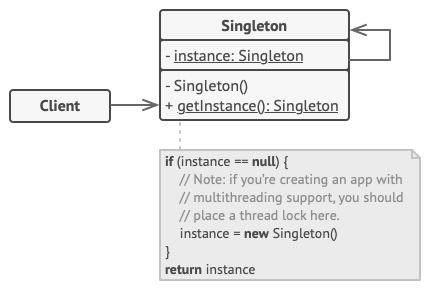
\includegraphics{../img/singleton.png}
\caption{Struktura jedinstveno instancirane klase}
\end{figure}

\hypertarget{mvvm-arhitektura}{%
\chapter{MVVM Arhitektura}\label{mvvm-arhitektura}}

Prvi put sam se susreo s MVVM arhitekturom GUI aplikacija. U početku sam
imao problema s granicom između \emph{pogleda} i \emph{modela pogleda},
no do kraja izrade prve verzije projekta sam dosta produbio
razumijevanje te arhitekture.

\textbf{Model} - sloj aplikacije zaslužan za definiranje podatkovnih
struktura aplikacije.

\textbf{Pogled (engl. View)} - sloj aplikacije zaslužan za slaganje i prikaz komponenti
s kojima korisnik interagira

\textbf{Model pogleda (engl. View Model)} - sloj aplikacije namijenjen
pohrani i manipulaciji modela, kao i definiranju izvora događaja za
reaktivnost

\hypertarget{nedostaci-aplikacije}{%
\chapter{Nedostaci aplikacije}\label{nedostaci-aplikacije}}

Trenutnoj implementaciji aplikacije nedostaje sljedeće:
\begin{itemize}
    \item Dijakritički znakovi nisu podržani.
    \item Ne postoji praćenje uspješno i neuspješno završenih partija.
\end{itemize}

\hypertarget{izrada-dijagrama}{%
\chapter{Izrada dijagrama}\label{izrada-dijagrama}}

Za izradu UML dijagrama klasa je bio korišten
\href{https://github.com/pierre3/PlantUmlClassDiagramGenerator}{PlantUmlClassDiagramGenerator
(autor: Hirotada Kobayashi)}; \href{https://staruml.io/}{PlantUML}
\href{https://github.com/staruml/staruml-csharp}{C\# import} i
\href{https://apps.kde.org/umbrello/}{Umbrello} nisu radili.
    

\begin{landscape}
\chapter{UML Dijagrami}

\begin{figure}[!hp]
\centering
\vfill
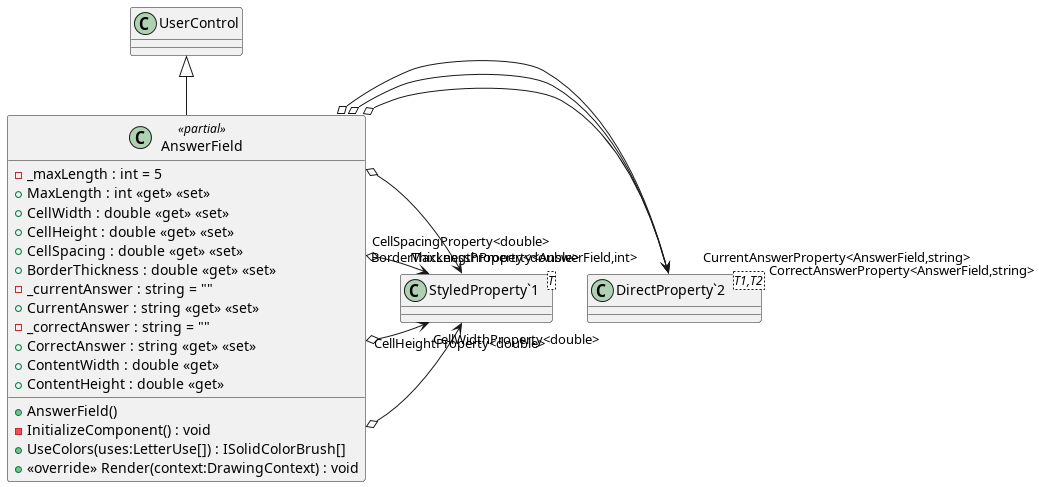
\includegraphics[width=\textwidth,height=\textheight,keepaspectratio]{../PlantUML/Components/include.png}
\vfill
\caption{Dijagram komponenta}
\end{figure}
\newpage

\begin{figure}[p]
\centering
\vfill
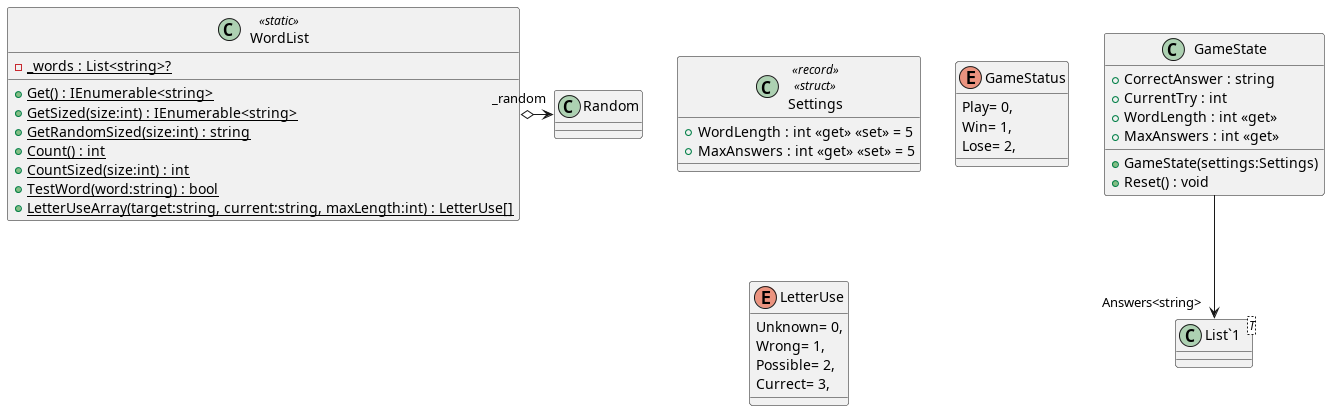
\includegraphics[width=\textwidth,height=\textheight,keepaspectratio]{../PlantUML/Model/include.png}
\caption{Dijagram modela}
\vfill
\end{figure}
\newpage

\begin{figure}[p]
\centering
\vfill
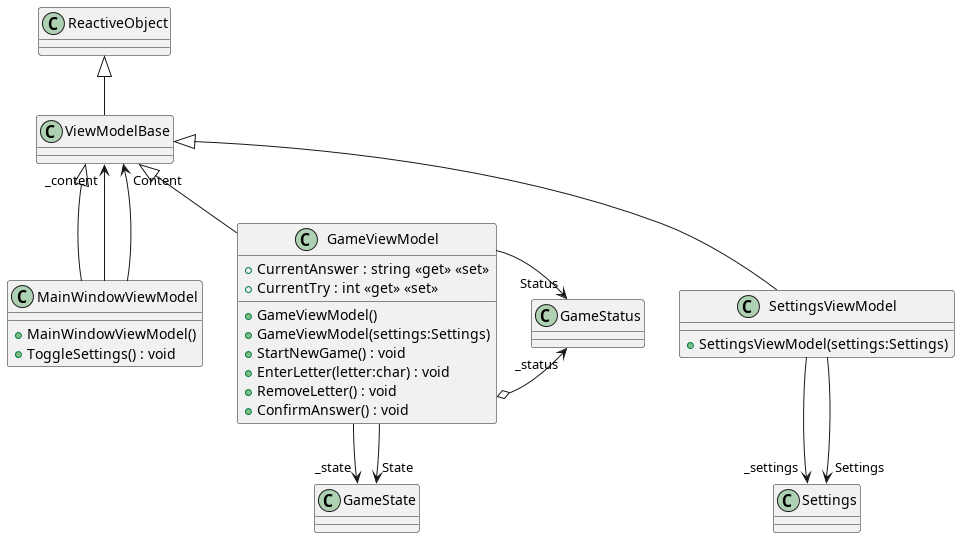
\includegraphics[width=\textwidth,height=\textheight,keepaspectratio]{../PlantUML/ViewModels/include.png}
\caption{Dijagram pogled-komponenta}
\vfill
\end{figure}
\newpage

\begin{figure}[p]
\centering
\vfill
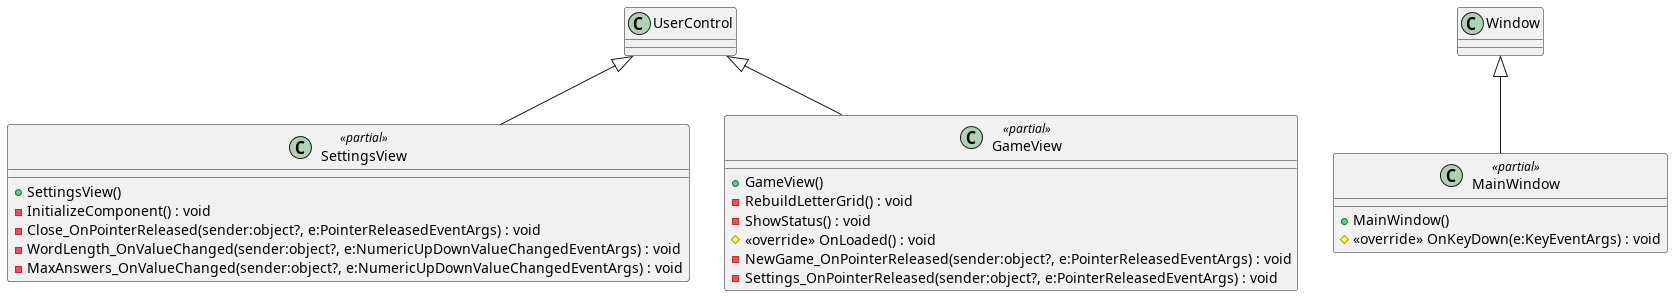
\includegraphics[width=\textwidth,height=\textheight,keepaspectratio]{../PlantUML/Views/include.png}
\caption{Dijagram pogleda}
\vfill
\end{figure}
\newpage

\end{landscape}

\end{document}
